\documentclass[titlepage, letterpaper,12pt]{article}
\usepackage[utf8]{inputenc}
\usepackage{booktabs}
\usepackage{tabularx}
\usepackage{makecell}
\usepackage{graphicx}
\usepackage{svg}
\usepackage{caption}
\usepackage{wrapfig}

\graphicspath{{./figs/}}
\def\svgwidth{\textwidth}

\renewcommand{\theadalign}{bl}
\renewcommand\theadfont{\bfseries}

\newcommand{\itwoc}{I\textsuperscript{2}C}


%opening
\title{Modular Electric Skateboard}
\author{Nick Fajardo, Phillip Konyeaso, Zane Weissman}

\begin{document}

\maketitle

\tableofcontents
\listoffigures
\listoftables

\begin{abstract}
The Modular Electric Skateboard (MESB) is an electric skateboard (ESB) that allows the user to mix and match components tailored to a specific user’s needs. The MESB is equipped with a TBD watt motor controlled by a handheld RC controller and capable of acheiving speeds as high as TBD. The deck, the part of the board on which the user stands while riding, can be disassembled and reassembled by hand to swap out major mechanical components of the board. The board's electrical system includes rails for mounting hot-swappable accessories.

\end{abstract}

\section{Background}
There are many means of transportation available in cities; some are more time consuming than others. Though cars are nearly ubiquitous in America, bicycles, buses, and trains remain popular alternatives. Recently, electric skateboards have filled a particular niche for some travelers. They have the advantages of decent speed (often above 20 mph) and good portability but are often held back by low range, making them ideal for short rides and trips that include trains or buses as well. Electric skateboards and similar devices can take many forms; the market is still new, but most are recognizable as a skateboard or longboard with a motor and drive train, an enclosure for batteries and electronics, and a handheld speed controller which may be wired or wireles.
\subsection{Skateboard Parts and Terminology}
Skateboarding has been around since the mid 1900s, and has changed drastically since its inception. Figures \ref{parts1} and \ref{parts2} show the different parts that make a modern complete skateboard, and the list below defines each part in detail.
\begin{figure}[!htbp]\centering
\begin{minipage}{.5\textwidth}\centering
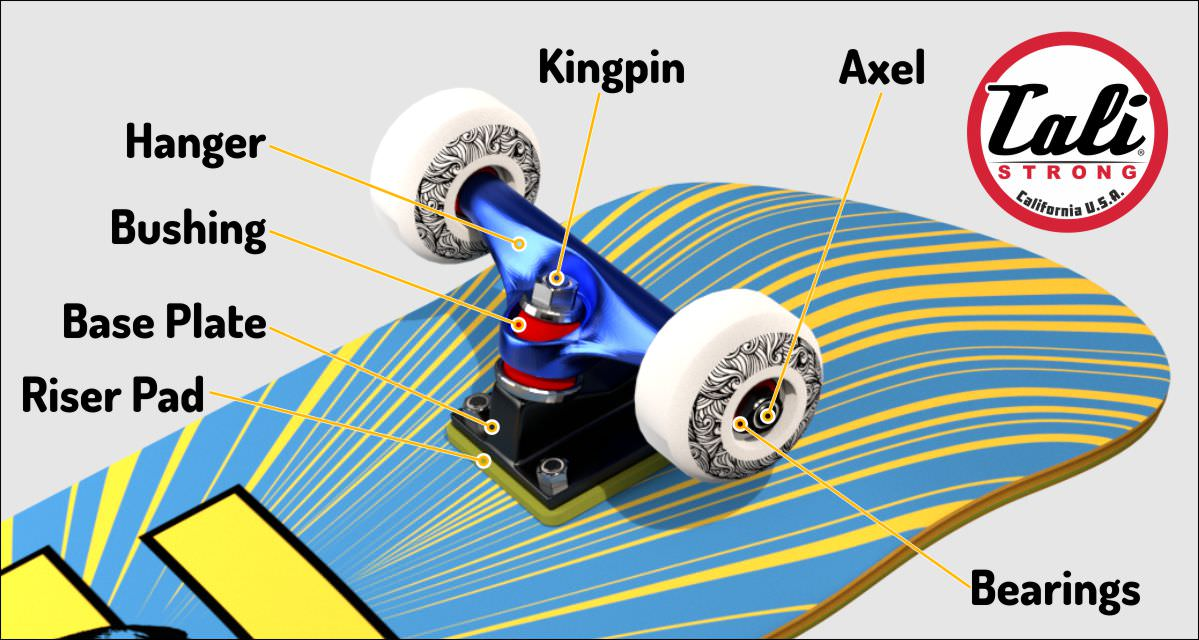
\includegraphics[width=.8\textwidth]{parts1.jpg}
\captionof{figure}{Skateboard Parts}
\label{parts1}
\end{minipage}%
\begin{minipage}{.5\textwidth}\centering
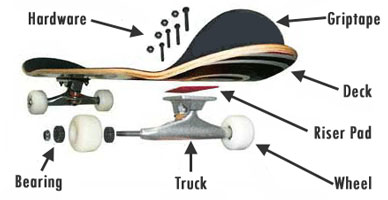
\includegraphics[width=.8\textwidth]{parts2.jpg}
\captionof{figure}{Skateboard Parts}
\label{parts2}
\end{minipage}
\end{figure}

\begin{itemize}
\item Deck - The surface on which the rider stands and to which the trucks and griptape are attached. It is essential for any deck to be sturdy, but also have some amount of flex for comfort. Decks vary in size and material, but they are typically wooden and a few feet long.
\begin{itemize}
\item Griptape - An adhesive surface for the top of the deck. One side is a very strong tape; the other side is a rough, sandpaper-like surface designed for high friction with the soles of the rider's shoes. Griptape comes in different grits (measure of “roughness”) and colors, but it is most often black.
\item Nose - Front of the board. A typical skateboard has a nose that is angled up.
\item Tail - Rear of the board. A typical skateboard has a tail that is angled up.
\end{itemize}
\item Trucks - The assemblies that connect the wheels to the deck.
\begin{itemize}
\item Hanger - The main, T-shaped portion of the truck.
\item Riser Pad - A pad used to add distance between the wheel and the deck. Often made of a material conducive to dampening vibration, such as rubber or cork.
\item Baseplate - The metal piece of the truck that is bolted to the deck. The rest of the truck sits on a threaded rod that extends downwards from the baseplate.
\item Bushings - Spacers between the kingpin, the hanger, and the base plate. Bushings can be replaced to adjust the force required to turn while riding; i.e., a bushing that is harder to compress will require the user to lean to a direction more in order to perform the same degree of turn as a softer to compress bushing. Often made of some sort of rubber polymer.
\item Kingpin - A nut, usually a locknut, used to cap the hanger and bushing assembly. It can be loosened and tightened to fine tune the hardness of its bushing.
\item Axel - The rod used to attach the wheels, typically integral to the hanger. Axel nuts hold screw onto the axel's threaded ends to hold the wheels in place.
\item Bearings - Assemblies that sit between the axels and wheels to ensure smooth rotation.
\item Wheels - Skateboard wheels, vary in size, shape, color, and material (though typically they are some type of relatively hard plastic), but most are interchangeable without changing any other parts. Size and material can have significant effects on shock absorption and the frictional forces between the wheels and the road; a new set of wheels can drastically change the way that a skateboard handles.
\end{itemize}
\item Hardware - All the nuts and bolts needed to attach the trucks to the deck.
\item Longboard - Type of skateboard more suited for traveling long distances. Longboard decks are elongated and often somewhat flexible or bouncy; longboard trucks are typically looser (i.e. requiring less force to turn).
\end{itemize}

\subsection{Board Shape}
Board shape can be split into multiple categories. First category is the deck shape, and the second is the concavity of the board. Taking both into consideration allowed the group to pick an ideal board to begin with for testing.

\subsubsection{Deck Shape}
Deck shape is important, because when longboarding the deck shape largely determines whether the board is meant for cruising or downhill. The two standard types are shown in the images below.
\begin{figure}[!htbp]\centering
\begin{minipage}{.5\textwidth}\centering
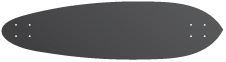
\includegraphics[width=.8\textwidth]{cruiser.jpg}
\captionof{figure}{Cruiser}
\label{cruiser}
\end{minipage}%
\begin{minipage}{.5\textwidth}\centering
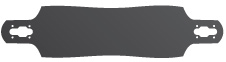
\includegraphics[width=.8\textwidth]{downhill.jpg}
\captionof{figure}{Downhill}
\label{downhill}
\end{minipage}
\end{figure}
\begin{itemize}
\item Cruisers - This is the most popular longboard style, and the deck size allows for greater weight distribution. It is reliable, however they usually aren't stiff and have shorter wheelbases compared to downhill decks. Their main purpose is riding on flat ground comfortably and quickly.

\item Downhill - As the name implies, this board type is for riding downhill quickly. It is important that deck doesn't flex much, and has a wide wheelbase otherwise the rider could lose control easily and become injured. It is usually advised to wear protective gear while riding these boards, because speeds when going downhill are very dangerous, and often lethal.

\end{itemize}

\subsubsection{Concavity}
Below are a types of concavity on the board. For the most part it is up to the user, and how he/she prefers the deck to feel under his/her feet.

\begin{itemize}

\begin{figure}[!htbp]\centering

\begin{minipage}{.5\textwidth}\centering
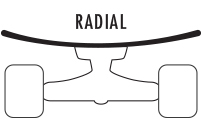
\includegraphics[width=.8\textwidth]{radial.jpg}
\captionof{figure}{Radial}
\label{radial}
\end{minipage}
\item Most Common Design, accepted relatively universally. The deeper the curve the better the feel of the board.
\end{figure}

\begin{figure}[!htbp]\centering
\begin{minipage}{.5\textwidth}\centering
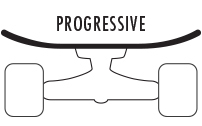
\includegraphics[width=.8\textwidth]{progressive.jpg}
\captionof{figure}{Progressive}
\label{progressive}
\end{minipage}
\item Similar to radial decks, but provides a more locked in feel with more secure footing.
\end{figure}

\begin{figure}[!htbp]\centering
\begin{minipage}{.5\textwidth}\centering
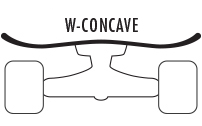
\includegraphics[width=.8\textwidth]{w-concave.jpg}
\captionof{figure}{W-Concave}
\label{w-concave}
\end{minipage}
\item Easier shifting of weight from foot to heel, highly precise and responsive deck.
\end{figure}

\begin{figure}[!htbp]\centering
\begin{minipage}{.5\textwidth}\centering
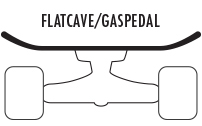
\includegraphics[width=.8\textwidth]{flatcave.jpg}
\captionof{figure}{Flatcave}
\label{flatcave}
\end{minipage}
\item Provides a more relaxed ride, but because of curved sides can apply some sudden shifts in weight.
\end{figure}

\begin{figure}[!htbp]\centering
\begin{minipage}{.5\textwidth}\centering
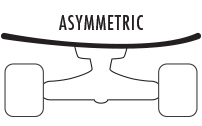
\includegraphics[width=.8\textwidth]{asymmetric.jpg}
\captionof{figure}{Asymmetric}
\label{asymmetric}
\end{minipage}
\item This board is good for riders who heavily rely on their heels to shift weight.
\end{figure}

\begin{figure}[!htbp]\centering
\begin{minipage}{.5\textwidth}\centering
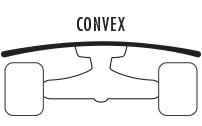
\includegraphics[width=.8\textwidth]{convex.jpg}
\captionof{figure}{Convex}
\label{convex}
\end{minipage}
\item Provides natural foot placement, but not as easy to control or safe.
\end{figure}

\begin{figure}[!htbp]\centering
\begin{minipage}{.5\textwidth}\centering
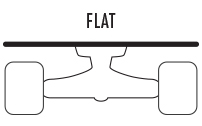
\includegraphics[width=.8\textwidth]{flat.jpg}
\captionof{figure}{Flat}
\label{flat}
\end{minipage}
\end{figure}
\item Allows for plenty of space for feet, and interesting tricks like boardwalking, which cannot be done easily on other decks.
\end{itemize}

\subsection{Electric Skateboards}
An electric skateboard (ESB) is a skateboard with one or more electric motors and drive trains attached to one or more wheels. The battery that powers the motor(s) is generally fixed to the bottom of the deck in a shroud that protects it and accompanying electronics from damage. The motor is often controlled with a handheld controller which may be wireless or wired. Alternatively, some ESBs include pressure or strain sensors in the deck and use the rider's balance to control the motor. ESBs are usually longboards, as they tend to provide smoother rides at the higher speeds often achieved with the electric motor.\\
One example of a relatively standard ESB is the Boosted Board brand “Dual+ XR” pictured in figure \ref{boosted}, which happens to also be one of the most popular off the shelf ESBs on the market today.
\begin{figure}[!htbp]\centering
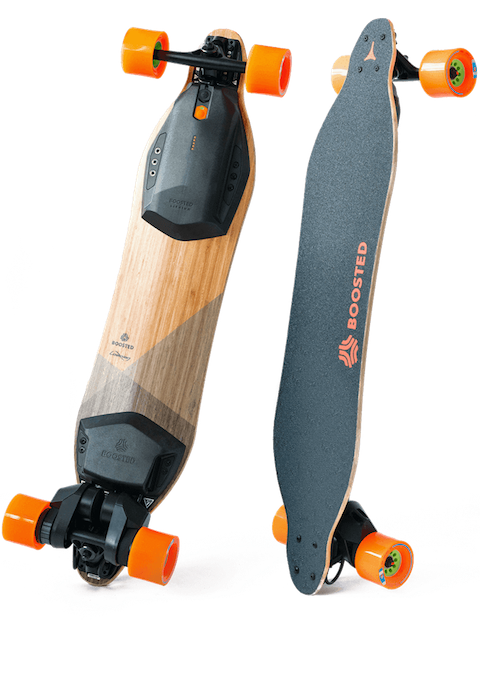
\includegraphics[width=.3\textwidth]{boosted.png}
\caption{Boosted Board Dual+ XR}
\label{boosted}
\end{figure}
It retails for \$1,599 and claims a top speed of 22 mph and a range of 14 miles with its 2000W motor and regenerative braking. Some more examples of popular ESBs can be found in table \ref{esbs}.
\begin{table}[!htbp]
\caption{Popular ESBs on the Market}
\label{esbs}
\resizebox{\textwidth}{!}{
\begin{tabular}{>{\bfseries}l l l l l}
\toprule
Board Name & Top Speed (mph) & Battery Range (miles) & Weight (lbs) & Price (Dollars) \\\hline
Inboard M1 & 22 & 7 & 14.5 & 1,000 \\
Boosted Plus/Stealth & 22/24 & 14 & 17 & 1,399/1.599 \\
Blink Qu4tro & 23 & 22 & 24 & 1,699 \\
Boosted Mini S/X & 18/20 & 7/14 & 15/16.8 & 749/999 \\
Onewheel +/+XR & 19 & 5-7/12-18 & 25 & 1,399/1,799 \\
\bottomrule
\end{tabular}
}
\end{table}

\section{System Overview}
The modular electric skateboard is an electric skateboard with a deck comprised of multiple sections which can be interchanged and replaced, a handheld remote controller for controlling the electric motor, a rail/data bus system attached to the underside of the deck which is capable of housing a number of accessories, and a small computer system which manages those accessories via a simple but flexible API.

\subsection{Mechanical Systems}
\subsubsection{Board and Linkages}
When thinking about the production of the board, in order to increase modularity the group thought that it would be beneficial to split the board into tips and a centerpiece. This would allow for users to attach different peripherals to the MESB as well as provide a simple access hub for which people who are interested in starting DIY to also be able to have an easy time changing parts. The board has two V-shaped cuts separating the tips from the center piece as shown in \ref{board-cut} as seen further below. Because of this feature, supporting linkages were needed in order to connect the pieces and improve stability. The final result we decided on was a double-v link, that faces the opposite direction of the cut. An example of a V-link can be seen in Figure \ref{singlev} of Statics Analysis.

\begin{figure}[!htbp]\centering
\begin{minipage}{.5\textwidth}\centering
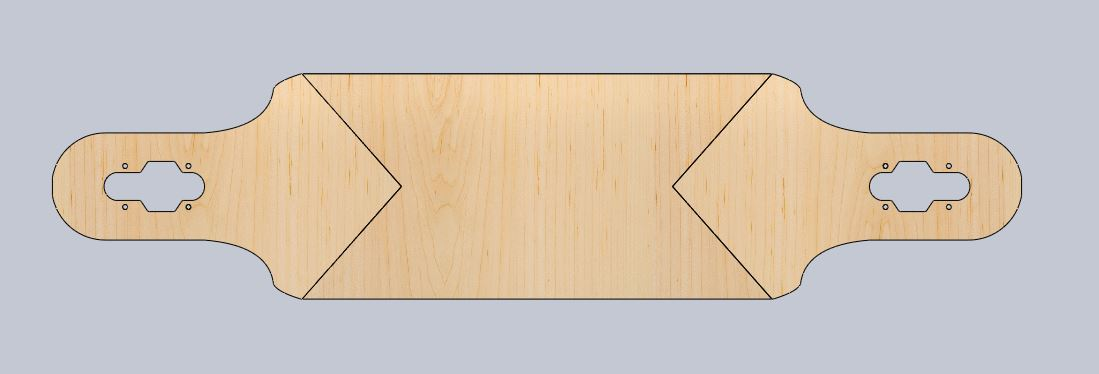
\includegraphics[width=.8\textwidth]{board-cut.JPG}
\captionof{figure}{board-cut}
\label{board-cut}
\end{minipage}
\end{figure}

\subsubsection{Modular Components}
The board is equipped with two modular housing "units". These units conform to the shape of the board, and are mounted with four bolts that span the length of the board, as shown in the figure below.

\begin{figure}
    \centering
    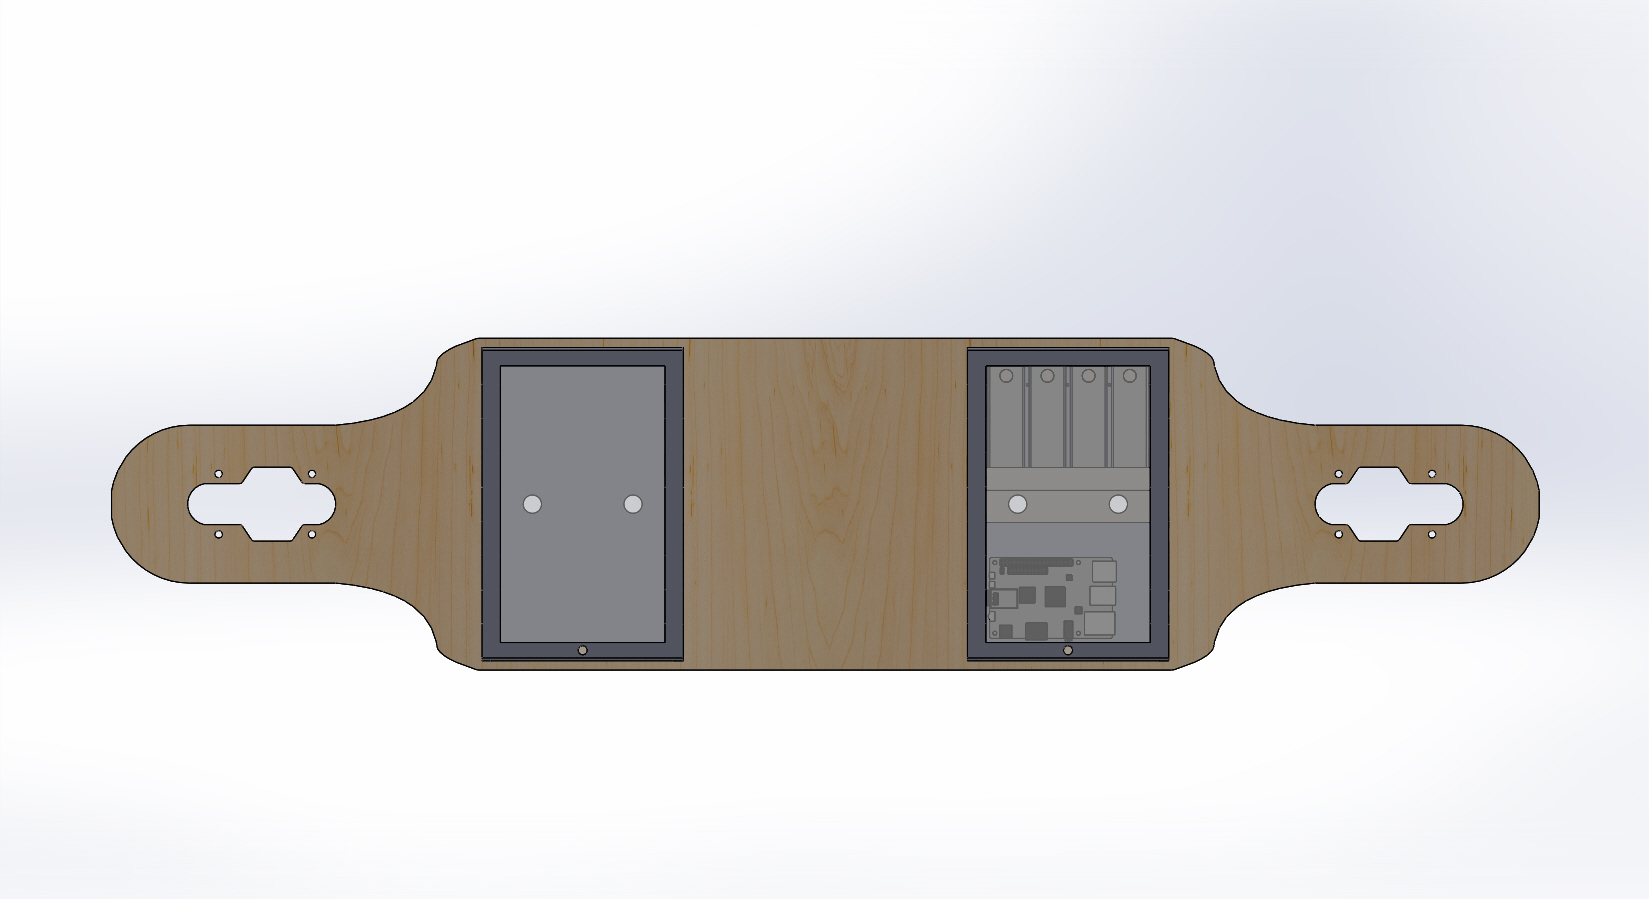
\includegraphics[width=10cm]{figs/ModularAssembledBottom.JPG}
    \caption{Board with Modular Components in Line}
    \label{inline}
\end{figure}

These units are placed in specific spots in order to accommodate for certain aspects of the system design. For instance, the component (referencing Figure \ref{inline}) to the left will house the batteries and electronics for the drive system. This is done since the skateboard will have a drive system only in the rear of the board, and placing the batteries and real time system closer to the drive will reduce the size of cables between them, which will impact likely hood of components being affected during use. The component on the right houses the customizable components of the board. These components will have a variety of uses in order to add functionality to the board, which can vary from the following list:

\begin{itemize}
    \item GPS Functionality
    \item Sensor Pack (IMU unit)
    \item Lighting System
    \item Storage Compartment
    \item Wireless Capabilities - Bluetooth/Wifi
\end{itemize}

\subsection{Control Systems and Control Processing}
Figure \ref{ctrl-overview} outlines the general structure of the motor control system.

%\includesvg[width=\textwidth]{rt}
%\input{figs/rt.pdf_tex}
\begin{figure}[!htbp]\centering
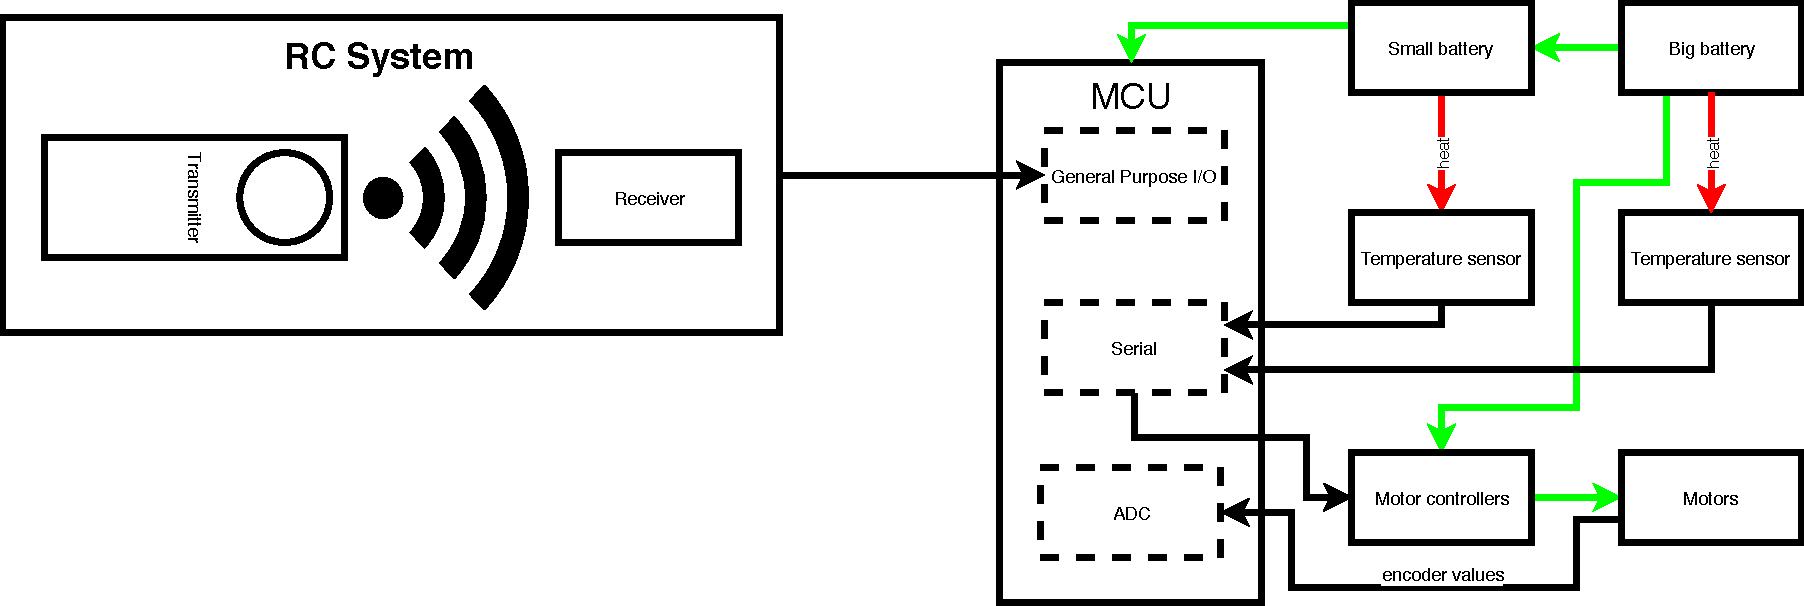
\includegraphics[width=\linewidth]{rt.pdf}
\caption{Major Components of Motor Control System}
\label{ctrl-overview}
\end{figure}
The remote control (RC) system is a standard 2.4 GHz hobbyist system designed for small unmanned RC cars and boats and comprised of a handheld transmitter, pictured in figure \ref{ctrl-tx}, and a small receiver which is attached to the vehicle being controlled.
\begin{figure}[!htbp]\centering
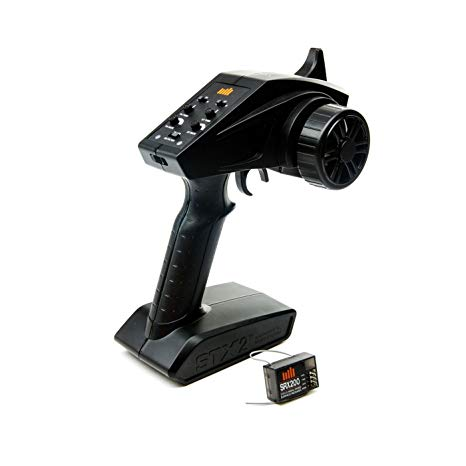
\includegraphics[width=0.5\textwidth]{controller.jpg}
\caption{Standard RC Transmitter and Receiver}
\label{ctrl-tx}
\end{figure}
The RC receiver outputs a pulse position modulation (PPM) signal that encodes the position of the throttle on the transmitter. This signal is read by the microcontroller (MCU). The MCU uses a PID control loop with throttle values, the temperatures of the primary and secondary batteries, and motor encoder readings as its inputs to determine the speed at which to drive the motors. The MCU software is structured as shown in figure \ref{mcu-sw}.
\begin{figure}[!htbp]\centering
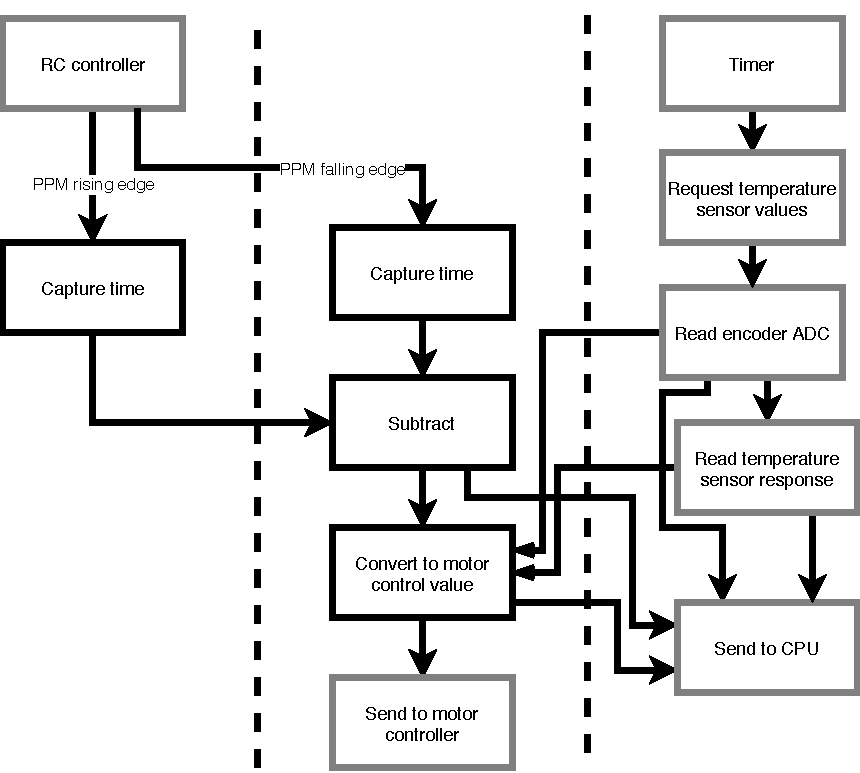
\includegraphics{mcusoftware.pdf}
\caption{Microcontroller Software Overview}
\label{mcu-sw}
\end{figure}

Each column represents a subroutine called by a hardware interrupt. In the case of the first two subroutines, the interrupt is triggered by the rising and falling edge, respectively of the PPM signal. On  the rising edge, a timer's value is captured. On the falling edge, the timer's value is captured again, and the difference between the times is the pulse position in which the throttle value is encoded. On each falling edge, an updated motor control value is decided based on the throttle position and based on encoder and temperature sensor values collected by a third interrupt routine and stored in global memory. The third routine is triggered at regular time intervals and collects temperature sensor and encoder values and sends them over a serial connection to the secondary computer system for long term storage.
\subsection{Electrical and Power Systems}
\subsubsection{Low Voltage Power}
The low voltage power system powers the MSP430 microcontroller, the Rock64 mini-PC, and any electronic accessories. Its main components are a battery comprised of two lithium cells for a total voltage of about 7.4 volts and a custom high-current voltage regulator that regulates to 5V. This regulator provides sufficient power to the MSP430 and Rock64, and can provide up to 2A at 5V to each accessory. For more information, see \ref{power-lv-sec}
\subsection{Computer and Accessory System}
Accessories are held in the dust resistant, water resistant (IP 66, see section for more details shrouds mounted to the underside of the deck, which also contain other electronic systems. Figure \ref{access-full} shows the shrounds mounted on the deck, while figure \ref{access-expl} shows an exploded view of the shroud itself.
\begin{figure}\centering
  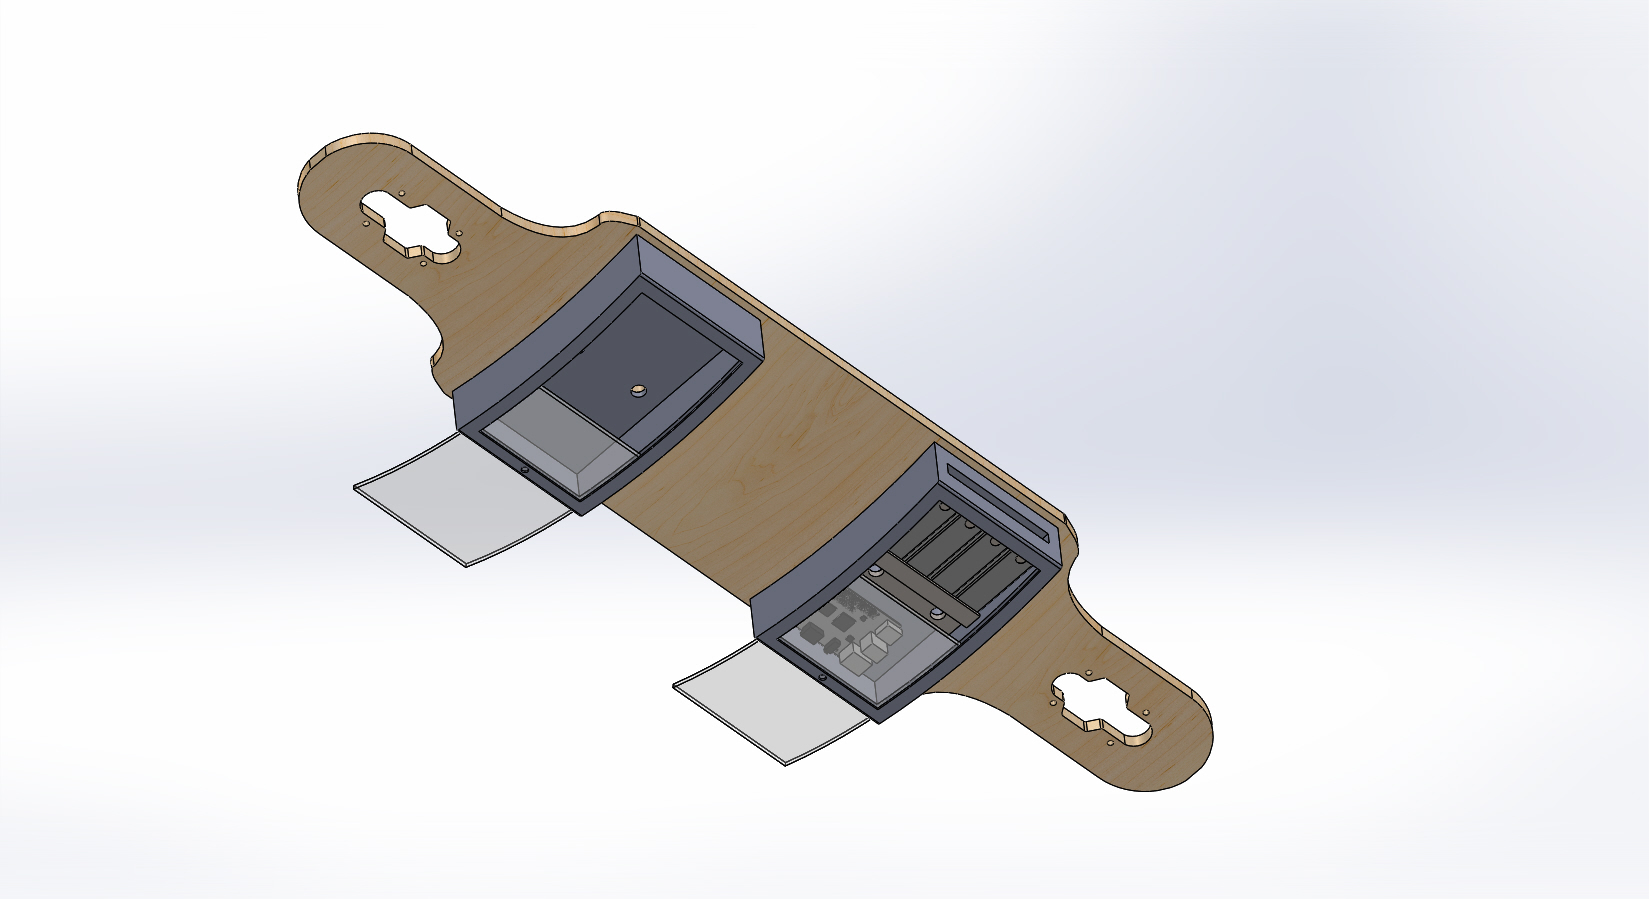
\includegraphics[width=.7\linewidth]{ModularAssembledBottomAngle}
  \caption{Electronics Shrouds}
  \label{access-full}
\end{figure}
\begin{figure}\centering
  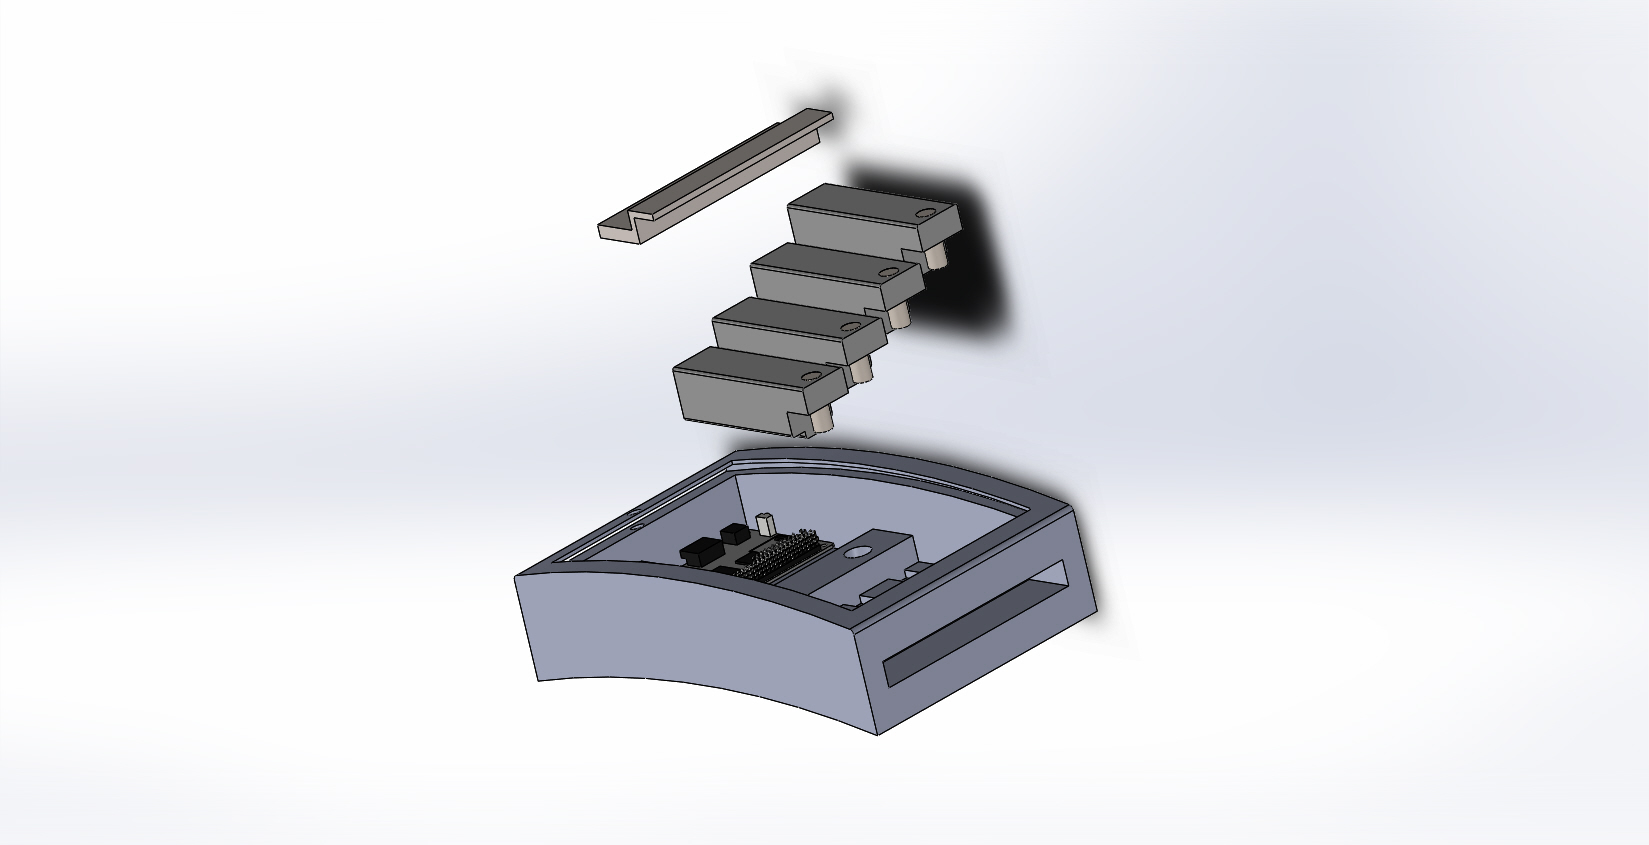
\includegraphics[width=.7\linewidth]{ModPieceAngleExtend}
  \caption{Exploded View of Accessory System in Shroud}
  \label{access-expl}
\end{figure}
Accessories slot into the base of the shroud, and then the horizontal beam is bolted on top of them to secure them during use. On the end opposite the beam is the accessory's Mini-DIN plug (for more detail, see \ref{access-plug}), used for power and data, which plugs into a port mounted to a PCB mounted to the shroud.

\section{Design Analysis}

\subsection{Mechanical System Analysis}
Representing the various elements of the Modular Electric Skateboard system requires a study on a variety of sections of the physical properties of the board. This includes calculating for the torque required to move the skateboard given its position, calculating the wheel contributions to a systems speed when a rotation around the board axis is induced, and using said calculations to derive the motors and gear ratios to use for the project.
\subsubsection{General Torque Calculations}
The system, in general, has a variety of physical properties that will not change during use.

% Table of system properties
\begin{table}[h]
\caption{Physical System Properties}
\begin{center}
 \begin{tabular}{||c c||}
 % \hline
 % Attribute & Numerical Value \\
 \hline
 Board Length & 39" \\
 \hline
 Board Width & 9.06" \\
 \hline
 Truck Width & 8.04" \\
 \hline
 High Friction Wheel Diameter & 2.625" \\
 \hline
 Low Friction Wheel Diameter & 2.48" \\
 \hline
\end{tabular}
\end{center}
\label{table:phys}
\end{table}

It is also important to note that the following assumptions are made during this analysis:
\begin{itemize}
    \item Wheel is inducing point contact on surface
    \item Rider and system mass are joined together, represented as a center of mass somewhere on the system
    \item There is no slippage
    \item Since we assume point contact, there will be no kinetic friction during movement
\end{itemize}

Using these properties, and a simple Free Body Diagram of the system, we can derive a general equation to map the motor torque and the acceleration on the given system.

\begin{figure}[h]
\caption{Free Body Diagram of System}
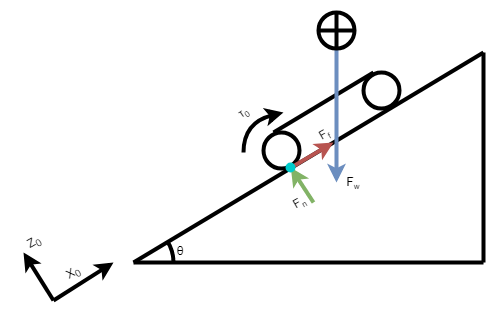
\includegraphics[width=8cm]{figs/FBD_MESB.png}
\centering
\end{figure}

\[\sum F _{x _{0}} = ma _x = F _f - \tau _{0} * R - F _wsin(\theta )\]
\[\sum F _{x _{0}} = ma _x = F _n \mu _s - \tau _{0} * R - F _wsin(\theta )\]
\[\sum F _{x _{0}} = ma _x = F _wcos(\theta) \mu _s - \tau _{0} * R - F _wsin(\theta )\]
\[\tau _{0} = \frac{a _x - gcos(\theta)\mu _s + gsin(\theta)}{-R \frac{1}{m}}\]

The torque that is required has a relation to the acceleration of the system in general at any given moment. We can convert this in terms of output motor torque:

\[\tau _0 = \tau _{motor}\mu_tT\]
\[\mu_t = transmission  \emph{ efficiency}\]
\[T = transmission \emph{ ratio}\]
\begin{equation} \label{eq:1}
    \tau _{motor} = \frac{a _x - gcos(\theta)\mu _s + gsin(\theta)}{-\mu_t T R \frac{1}{m}}
\end{equation}

Now we can map the motor torque to the acceleration of the body, which will help us calculate the necessary torque the motor needs to apply to the system given some sensor data and user input on requested speed.

\subsubsection{Wheel Contribution Calculations}
Equation \ref{eq:1} found a mapping between the board acceleration and motor torque, given some environment and system parameters. However, this case will only be accurate whenever the board torque is applied when a rotation around the board axis ($X _{0}$) is not present.

\begin{figure}[h]
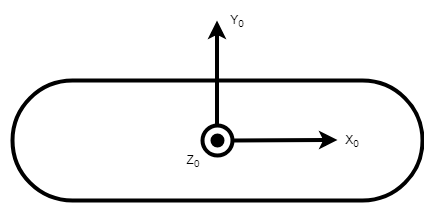
\includegraphics[width=8cm]{figs/Board_Axis.png}
\centering
\end{figure}

In cases when the user induces a turn on the axis, each wheel will contribute differently to the total board velocity, which is something that needs to be mathematically modeled in order to adjust speeds when inducing a rotation $\gamma$ along the $X _{0}$ axis. Please note that the following statements are valid and exploited in this derivation of wheel velocities:
\begin{itemize}
    \item Any $\gamma$ along $X _{0}$ induces a rotation angle along the front and rear trucks, and the angle on each truck is equal in magnitude, but opposite in direction.
    \item All wheels have the same properties
    \item We know the physical properties of the board, as specified in Table \ref{table:phys}
\end{itemize}

\begin{figure}[!h]
\caption{Position state by a rotation $\gamma$}
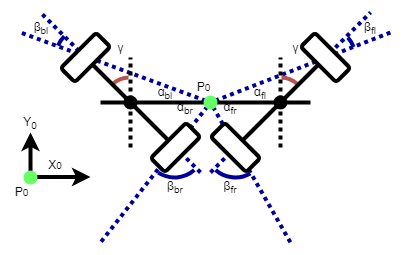
\includegraphics[width=10cm]{figs/Wheel_Reps.png}
\centering
\end{figure}

Assuming $\gamma$ is not zero, we can use the following relations to derive each wheel contribution:

\[L = \emph{distance from point P to center of wheel}\]
\[\vec{V} = \emph{Velocity of total body (relative to point P, in body frame)}\]
\begin{equation}
    \emph{Rolling Constraint} =
    [sin(\alpha + \beta), -cos(\alpha + \beta), -Lcos(\beta)]\vec{V} - r\dot{\delta} = 0
\end{equation}
\begin{equation}
    \emph{Sliding Constraint} =
    [cos(\alpha + \beta), sin(\alpha + \beta), Lsin(\beta)]\vec{V} - r\dot{\delta} = 0
\end{equation}

These relations are based off of alpha and beta, which can be found for each wheel using the known parameters

\begin{figure}[!h]
\caption{Position of Front Left Wheel}
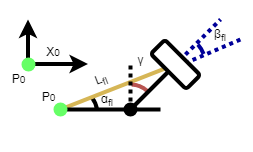
\includegraphics[width=10cm]{figs/FL.png}
\centering
\end{figure}

\begin{equation}
    \alpha _{fl} = cos^{-1}(\frac{\frac{T}{2}-L _{fl}^2-\frac{d}{2}^{2})}{-2L _{fl}\frac{d}{2}})
\end{equation}

\begin{equation}
    \beta _{fl} = cos^{-1}(\frac{\frac{d}{2}-L _{fl}^2-\frac{T}{2}^{2})}{-2L _{fl}\frac{T}{2}})
\end{equation}

Similar calculations can be performed on each wheel, which in the end will yield functions that map our board rotation and wheel speeds to the given board speed. We will summarize the process of combining the wheel velocity equations gathered from the process above and solving for the board velocity $\vec{V}$ inside a function:

\begin{equation}
    \vec{V} = mapRotationToSpeed(Board Rotation) = mapRV(\gamma)
\end{equation}

This will allow us to more accurately produce a body velocity to feed into a control system to then tell the board what torque to produce.

\subsection{Modular Platform}
When conceiving of the concept of how to attach modules on the board in a way that is friendly to the user, Picatinny Rails were the top option for most of the preliminary phase of the project. These rail systems allow any unit with a matching coupling device to be mounted to the rail system, and the device can vary in size with ought affecting the quality of the coupling system when under load.

On the skateboard, it would be places in areas that both are not prone to contact with the ground when the board is moving on uneven surfaces and places in an area that would not affect the structure of the board.

\begin{figure}[h]
    \centering
    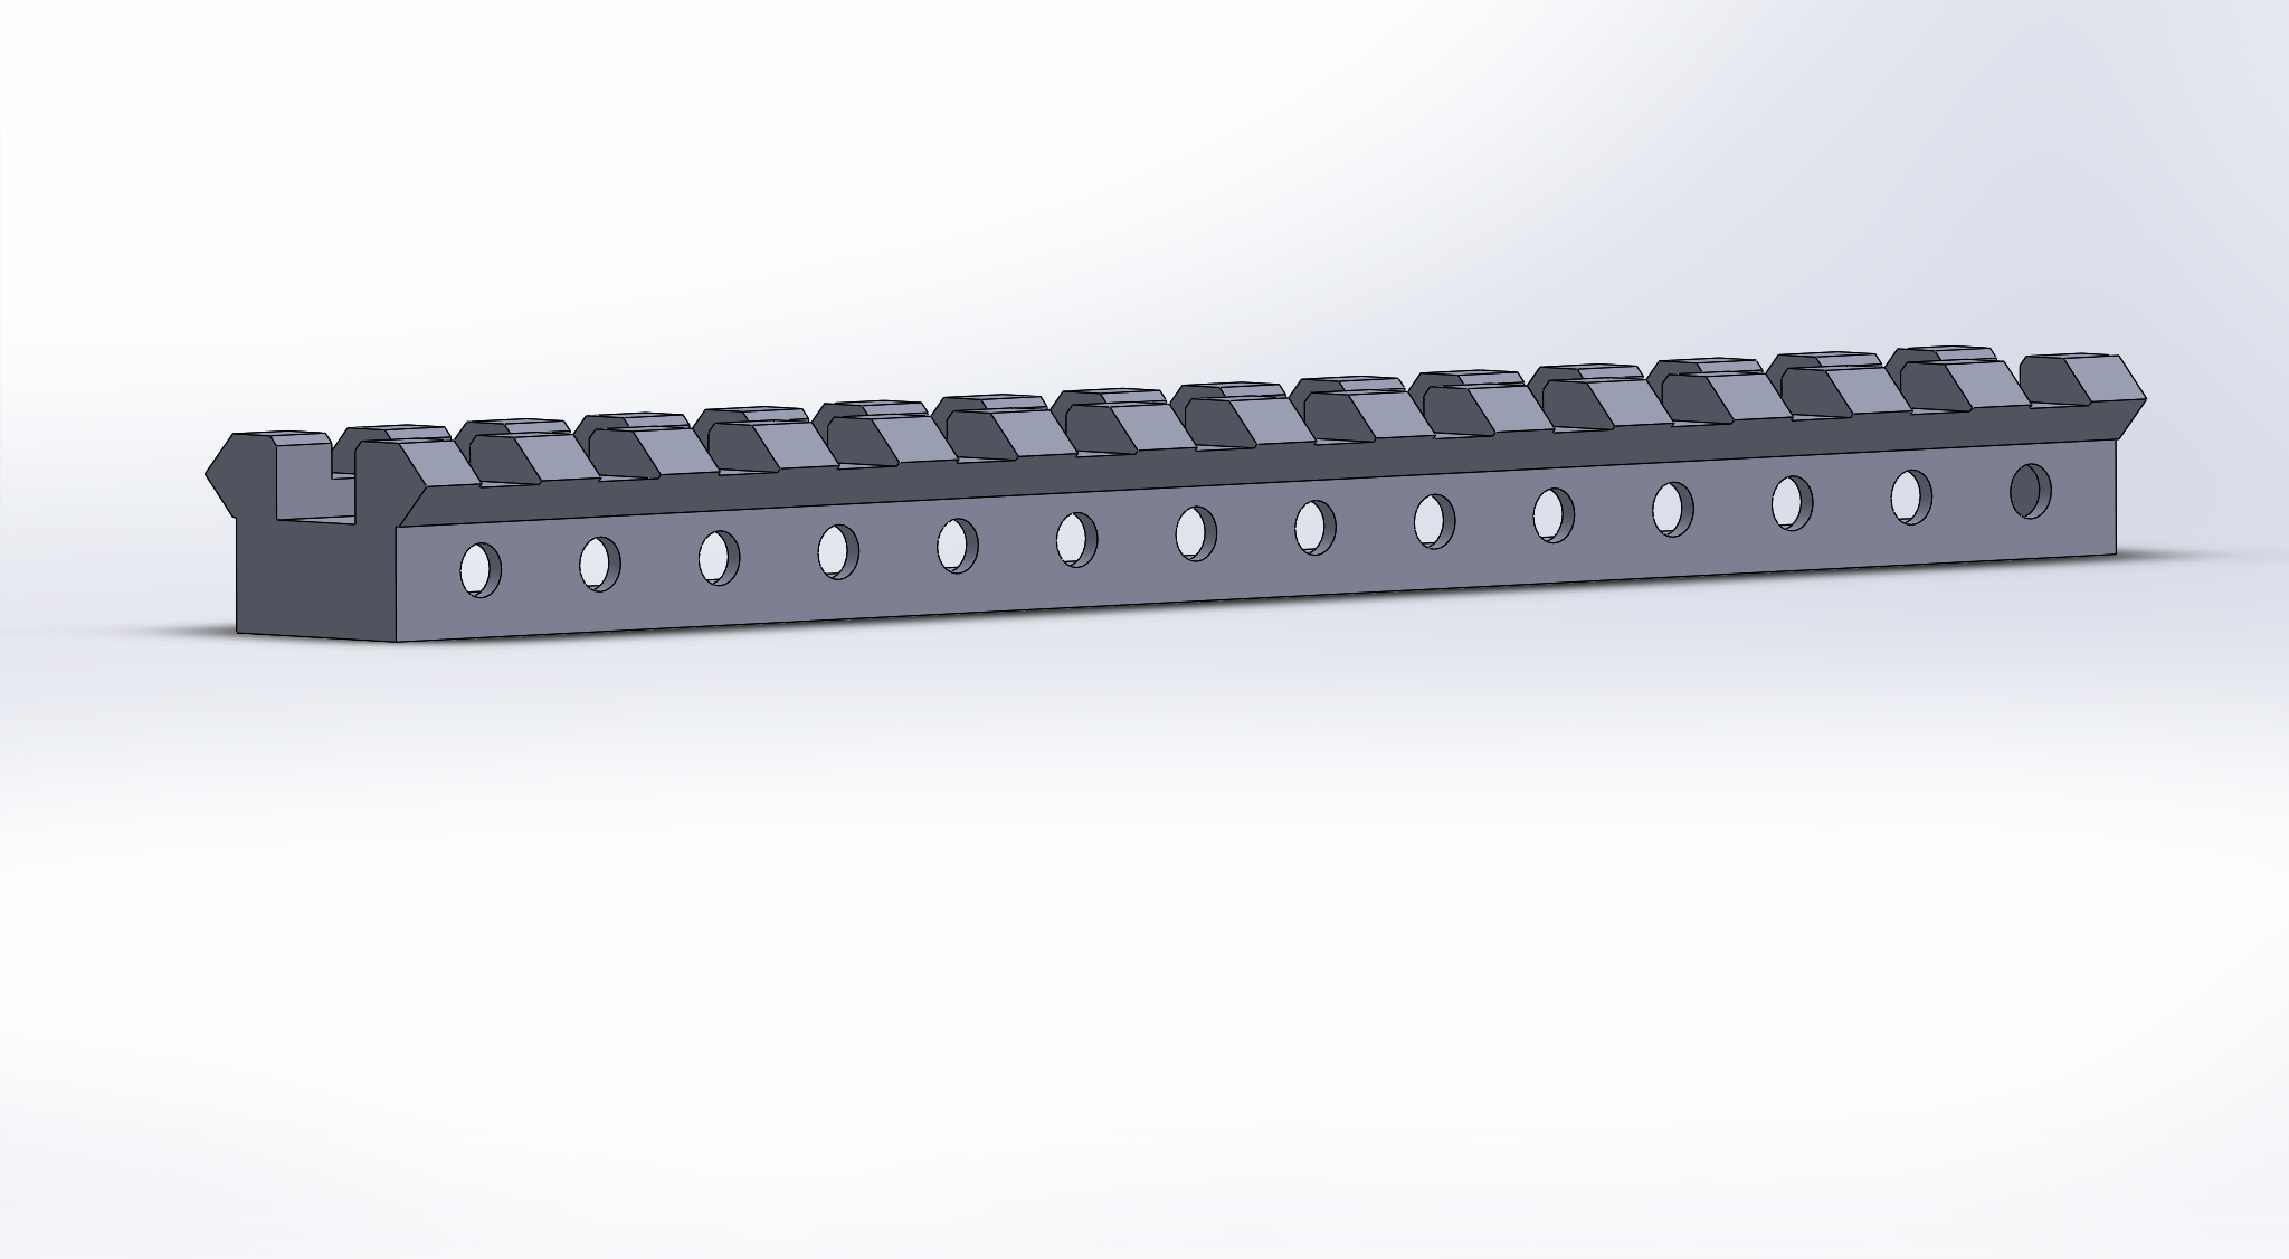
\includegraphics[width=10cm]{figs/Picatinny_Rail.JPG}
    \caption{Picatinny Rail}
    \label{fig:picTiny}
\end{figure}

After some thought and discussions with external personnel, we started to conceive of various modular systems that would be better to manufacture. This was done in order to look at the project from the point of view of the manufacturer, which would inheritly open up opportunities to fabricate a system that would implement smaller units under the deck of the board, and retain a higher standard for durability in terms of water resistance, shock, and other elements.

\begin{figure}[!h]
    \centering
    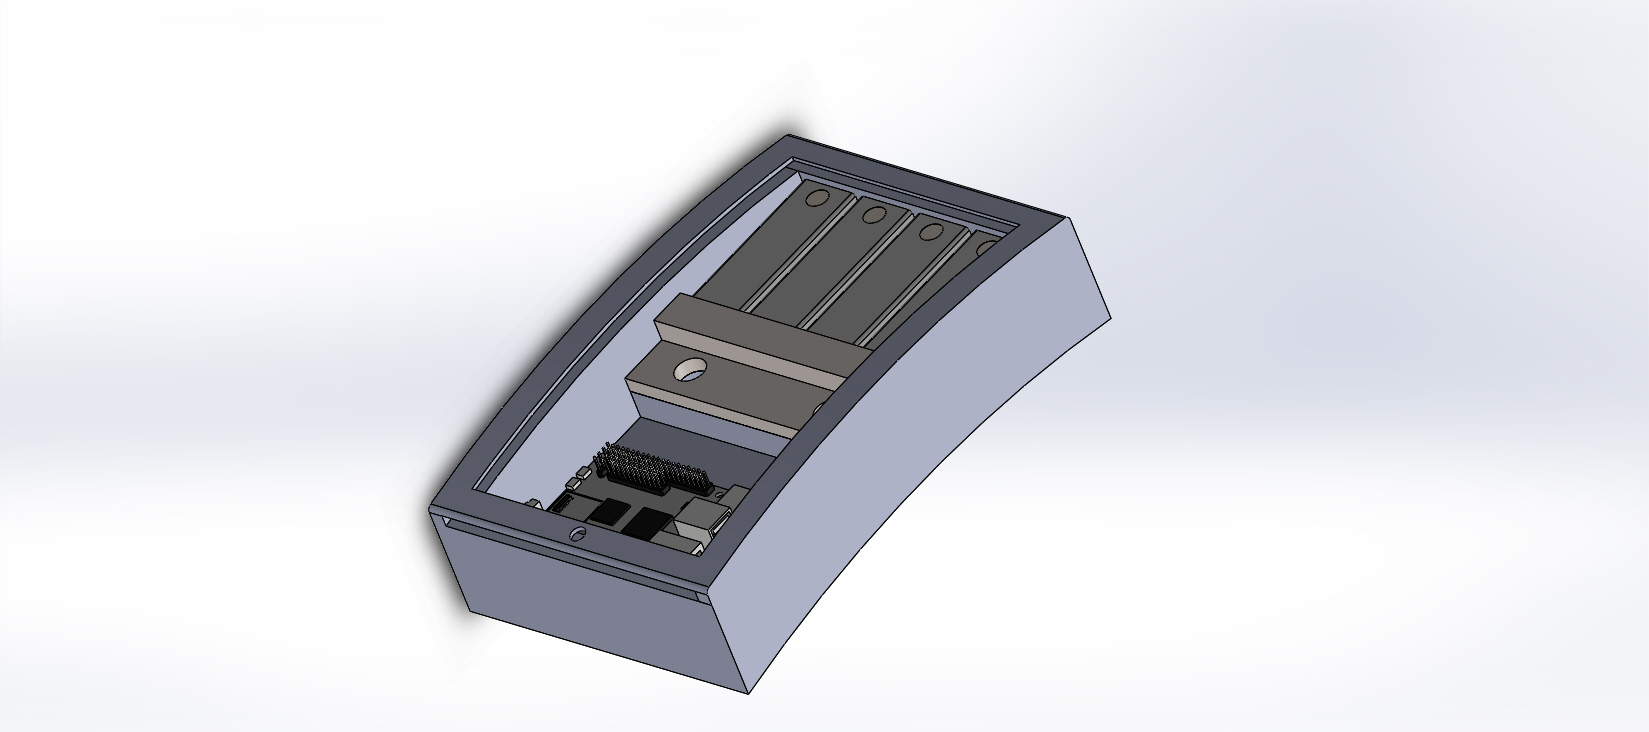
\includegraphics[width=10cm]{figs/ModPieceAngle.JPG}
    \caption{Modular Unit}
    \label{fig:picTiny}
\end{figure}

\begin{figure}[!h]
    \centering
    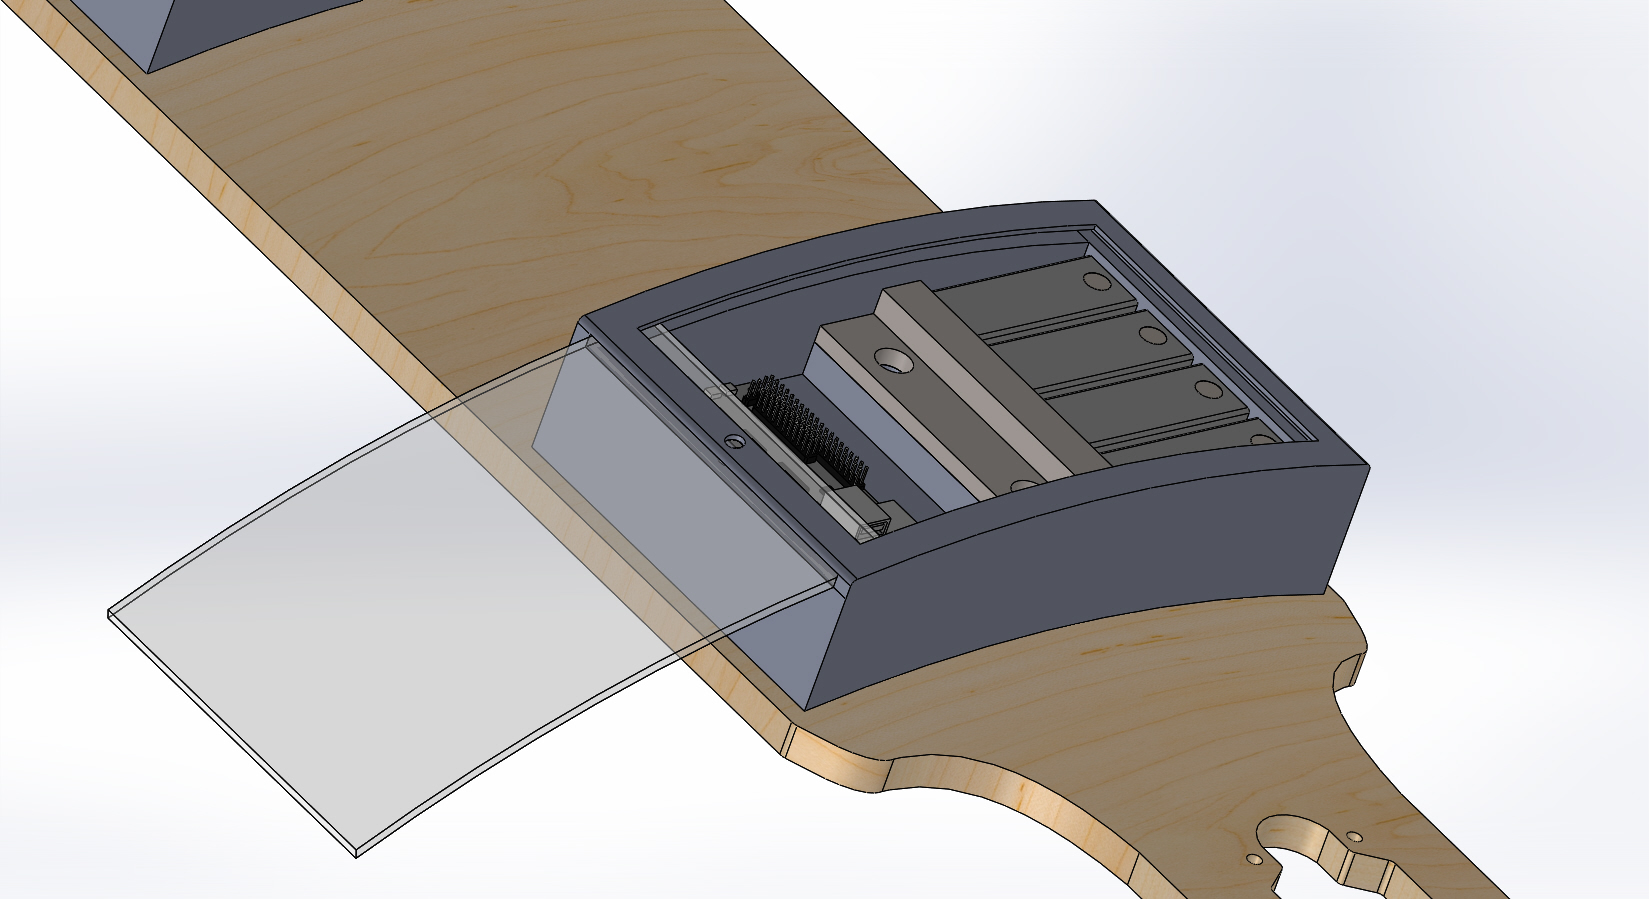
\includegraphics[width=10cm]{figs/ModularAssembledZoomModOpen.JPG}
    \caption{Modular Unit on board}
    \label{fig:picTiny}
\end{figure}


\subsection{Trade Studies}
This section breaks down in detail several tradeoffs of components, protocols, etc. which had to be considered once the system level design was finished. Each column compares the qualities of a certain attribute of the systems under study, and lists the point value score assigned to each quality. The maximum acheivable score in each category is listed in the header of each category with a ``/'' preceding it; the maximum acheivable total score is listed in the header of the leftmost column listing the names of the systems being compared.

\subsubsection{Real Time Microcontroller}
Before choosing a specific processor or development board, several microcontroller (MCU) platforms were compared. At least some variants of each of the microcontrollers in table \ref{tr-mcu} would meet the basic requirements of the MCU for the real time control system on the MESB, such as hardware interrupts and an appropriate number of analog to digital converters, timers, etc.
\begin{table}[!htbp]
\caption{Real Time Microcontroller Trade Study}
\label{tr-mcu}
\resizebox{\textwidth}{!}{
\begin{tabular}{>{\bfseries}l>{\bfseries}r lr lr lr lr lr}
\toprule
%platform & Total Points & Price & Points (5) & architecture & Points (4) & clock & Points (2) & current draw & Points (2) & Familiarity/ease of use & Points (6)
%\tradecat{Platform} & \tradecat{Price} \\
\thead{Platform} & /20 & \thead{Price} & /5 & \thead{Architecture} & /5 & \thead{Core \\ Clock} & /2 & \thead{Current \\ Draw } & /2 & \thead{Familiarity \\ \& Ease of Use} & /6\\
\cmidrule(r){1-2} \cmidrule(r){3-4} \cmidrule(r){5-6} \cmidrule(r){7-8} \cmidrule(r){9-10} \cmidrule(r){11-12}
%Name & Total Points & Price & Points\\
MSP430 & 16 & \$10-18 & 4 & 16 bit RISC & 3 & 8-24 MHz & 1 & ~5 mA & 2 & High & 6\\
STM32 Cortex & 13 & \$10-25 & 4 & 32 bit ARM Cortex-m & 4 & 32-400MHz & 2 & ~100-500 uA/MHz & 0 & Moderate & 3\\
ATMega328P & 15 & \$3-10 & 5 & 8 bit AVR RISC & 1 & up to 20 MHz & 1 & ~5 mA & 2 & High & 6\\
\bottomrule
\end{tabular}
}
\end{table}
Though all of these platforms had their advantages and disadvantages, the MSP430 was chosen for its capable and flexible 16-bit architecture, its low cost and power consumption, and for the developers' familiarity with the ins and outs of its hardware and firmware.

Table \ref{tr-msp} compares various MSP430 development boards. The names are truncated to avoid redundancy and save space; the development boards being compared are the MSP-EXP430FR2355, MSP-EXP430FR2433, etc., using the MSP430FR2355, MSP430FR2433, etc. microprocessors, respectively.\\
\begin{table}[!htbp]
\caption{MSP430 Trade Study}
\label{tr-msp}
\resizebox{\textwidth}{!}{
\begin{tabular}{>{\bfseries}l>{\bfseries}r lr lr lr lr lr}
\toprule
\thead{MCU} & /15 & \thead{Price}& /8 & \thead{Core Clock} & /2 & \thead{RAM + \\ Storage} & /5 & \thead{Current Draw} & /3 & \thead{ADCs} & /2 \\
\cmidrule(r){1-2} \cmidrule(r){3-4} \cmidrule(r){5-6} \cmidrule(r){7-8} \cmidrule(r){9-10} \cmidrule(r){11-12}
FR2355 & 12 & \$13 & 5 & 24 MHz & 2 & 32KB & 2 & 142 uA/MHz,{\raise.5ex\hbox{$\scriptstyle\sim$}}1 uA standby & 1 & 1x12b & 2\\
FR2433 & 13 & \$10 & 8 & 16 MHz & 1 & 15.5KB & 1 & 125 uA/MHz; $<$1 uA standby & 2 &8x10b & 1\\
FR5994 & 11 & \$17 & 1 & 16 MHz & 1 & 264KB & 5 & 118 uA/MHz; 500 nA standby & 2 & 1x12b & 2\\
FR4133 & 10 & \$14 & 4 & 16 MHz & 1 & 15.5KB & 2 & 126 uA/MHz; $<$1 uA standby & 2 &10x10b &1\\
FR6989 & 10 & \$18 & 0 & 16 MHz & 1 & 128KB & 4 & 100 uA/MHz; 350 nA standby & 3 & 16x12b & 2\\
FR5969 & 11 & \$16 & 2 & 16 MHz & 1 & 62KB & 3 & 100 uA/MHz; .4 uA standby & 3 & 16x12b & 2\\
F5529 & 16 & \$13 & 5 & 25 MHz & 2 & 136KB & 4 & 150 uA/MHz; 2 uA standby & 3 & 1x12b & 2\\
\bottomrule
\end{tabular}
}
\end{table}
The MSP430F5529 offers above average MSP430 performance for below average price. While its higher clock rate may not be necessary, 128KB of flash memory provide a comfortable amount of program storage space
\subsubsection{Accessory Bus Serial Protocol}
Table \ref{tr-serial} compares several serial protocols which were considered for the main accessory bus:
\begin{table}[!htbp]
\caption{Accessory Bus Serial Protocol Trade Study}
\label{tr-serial}
\resizebox{\textwidth}{!}{
\begin{tabular}{>{\bfseries}l>{\bfseries}r lr lr lr lr }
\toprule
\thead{Name} & /27 & \thead{Wires, \\ Shared} & /3 & \thead{Add'l Wires \\ per Device }& /10 & \thead{Speed} & /4 & \thead{Ease\\ of Use} & /10\\
\cmidrule(r){1-2} \cmidrule(r){3-4} \cmidrule(r){5-6} \cmidrule(r){7-8} \cmidrule(r){9-10}
\itwoc & 25 & 2 & 2 & 0 & 10 & 100k-3.4Mbps & 3 & easy & 10\\
CAN & 17 & 2 & 2 & 0 & 10 & 1Mbps & 3 & hard & 2\\
SPI & 15 & 3 & 1 & 1 & 3 & 10Mbps & 4 & medium & 7\\
UART & 15 & 0 & 3 & 2 & 0 & {\raise.5ex\hbox{$\scriptstyle\sim$}}10-100kbps & 2 & easy  & 10\\
LIN & 17 & 1 & 3 & 0 & 10 & 20kbps & 1 & hard & 3\\
\bottomrule
\end{tabular}
}
\end{table}
\itwoc{} was chosen for its two-wire communication, ease of use, and more than sufficient speed. Some other serial protocols shared some but not all of these desirable attributes, but \itwoc{} scored nearly perfectly overall.

\subsubsection{Data Connector Plug and Socket}
Table \ref{tr-conn} compares several types of connectors which were considered for the data/power connections to accessories:
\begin{table}[!htbp]
\caption{Data Connector Trade Study}
\label{tr-conn}
\resizebox{\textwidth}{!}{
\begin{tabular}{>{\bfseries}l>{\bfseries}r lr lr lr lr lr lr lr lr lr }
\toprule
\thead{Name} & /21 & \thead{Data\\Lines} & /2 & \thead{Water\\Resistance} & /2 & \thead{Locking} & /2 & \thead{Terminal\\Area} & /3 & \thead{Terminal\\Length} & /3 & \thead{Price/\\Pair} & /3 & \thead{Strength} & /2 & \thead{Current\\(A)} & /2 & \thead{Voltage\\(V)} & /2\\
\cmidrule(r){1-2} \cmidrule(r){3-4} \cmidrule(r){5-6} \cmidrule(r){7-8} \cmidrule(r){9-10} \cmidrule(r){11-12} \cmidrule(r){13-14} \cmidrule(r){15-16} \cmidrule(r){17-18} \cmidrule(r){19-20}
TRRS 3.5mm & 15 & 2 & 2 & No & 1 & No & 1 & Small & 3 & Small & 3 & \$2-5 & 2 & Yes & 2 & 1 & 1 & 5 & 1 \\
Mini-DIN & 19 & 1-7 & 2 & Yes & 2 & No & 1 & Small & 3 & Small & 3 & \$2-5 & 2 & Yes & 2 & 2-7 & 2 & 30 & 2\\
Micro USB-B & 11 & 3 & 2 & Yes & 2 & No & 1 & Small & 3 & Small & 3 & \$3-7 & 1 & No & 1 & 2 & 2 & 5 & 1 \\
Mini USB-B & 19 & 3 & 2 & Yes & 2 & No & 1 & Small & 3 & Small & 3 & \$1 & 3 & Yes & 2 & 1 & 1 & 2-5 & 1 \\
4P4C & 18 & 2 & 2 &  Yes (IP67) & 2 & Yes & 2 & Small & 3 & Small & 3 & \$1 & 3 & Yes & 2 & 1 & 1 & 2-5 & 1 \\
8P8C & 19 & 6 & 2 &  Yes (IP67) & 2 & Yes & 2 & Small & 3 & Small & 3 & \$1 & 3 & Yes & 2 & 2 & 2 & 2-5 & 1 \\
DE-9 & 18 & 7 & 2 &  Yes & 2 & Yes & 2 & Large & 1 & Medium & 2 & \$1-2 & 2 & Yes & 2 & 5 & 2 & 100 & 2\\
\end{tabular}}
\end{table}
\subsection{Testing}
\subsubsection{Road Roughness and Ride Quality}
International standards for road roughness have existed for a few decades. Most commonly used is the international roughness index (IRI), a measure of the motion of a vehicle's suspension as it travels a certain distance over a road, reported in units of meters per kilometer or equivalently, millimeters per m. However, the assumed ``standard vehicle'' is a car, which of course has very different suspension characteristics from a skateboard, and furthermore, most cities do not regularly measure the IRI of their roads, nor are IRI measuring devices cheap or readily accessible, so measuring the IRI of a road or finding a road with a known IRI would be rather impractical. \\
Instead, roads in the neighborhood around Worcester Polytechnic Institute were categorized by simple subjective experience of riding a regular, unpowered longboard with the same deck which would then be used for the MESB. This provided, at the very least, a subjective baseline for the comfort and ease of riding on different types of roads, and a basic way to categorize roads based on the features that impact the feeling of the ride. The categories, with example streets, are as follows:
\begin{itemize}
 \item Freshly paved (Sever St): Top layer of asphalt still intact, covering the stones beneath. Ride is extremely smooth. Almost no vibration felt, no cracks or rough patches to avoid.
 \item Smooth (Somerset St, sidewalk around Elm Park): Asphalt in great condition, but the top layer has worn away and the small stones in the asphalt are visible. Noticeable vibration from the asphalt. Very few cracks or other issues.
 \item Medium (Dover, William): Asphalt is significantly rougher but not destroyed. Vibration is more substantial; there are many small cracks that can be felt when riding over them but that are not serious obstacles. Very few or no large cracks or potholes that would need to be avoided.
 \item Rough (Nicholas Fajardo’s driveway): Asphalt is rough to ride on with significant damage in some areas, including some that are impassable. Not possible to traverse at high speeds.
\end{itemize}
The MESB should be capable of traversing all of these types of terrain, even if it requires some caution, and it should be comparably comfortable to the stock longboard with the same deck.

\subsubsection{Low Voltage Power}\label{power-lv-sec}
A potential low voltage power system, for the microcontroller, CPU, and accessories, was designed in OrCAD Capture for simulation in PSpice. Figure \ref{power-lv} shows the circuit.
\begin{figure}[!htbp]\centering
  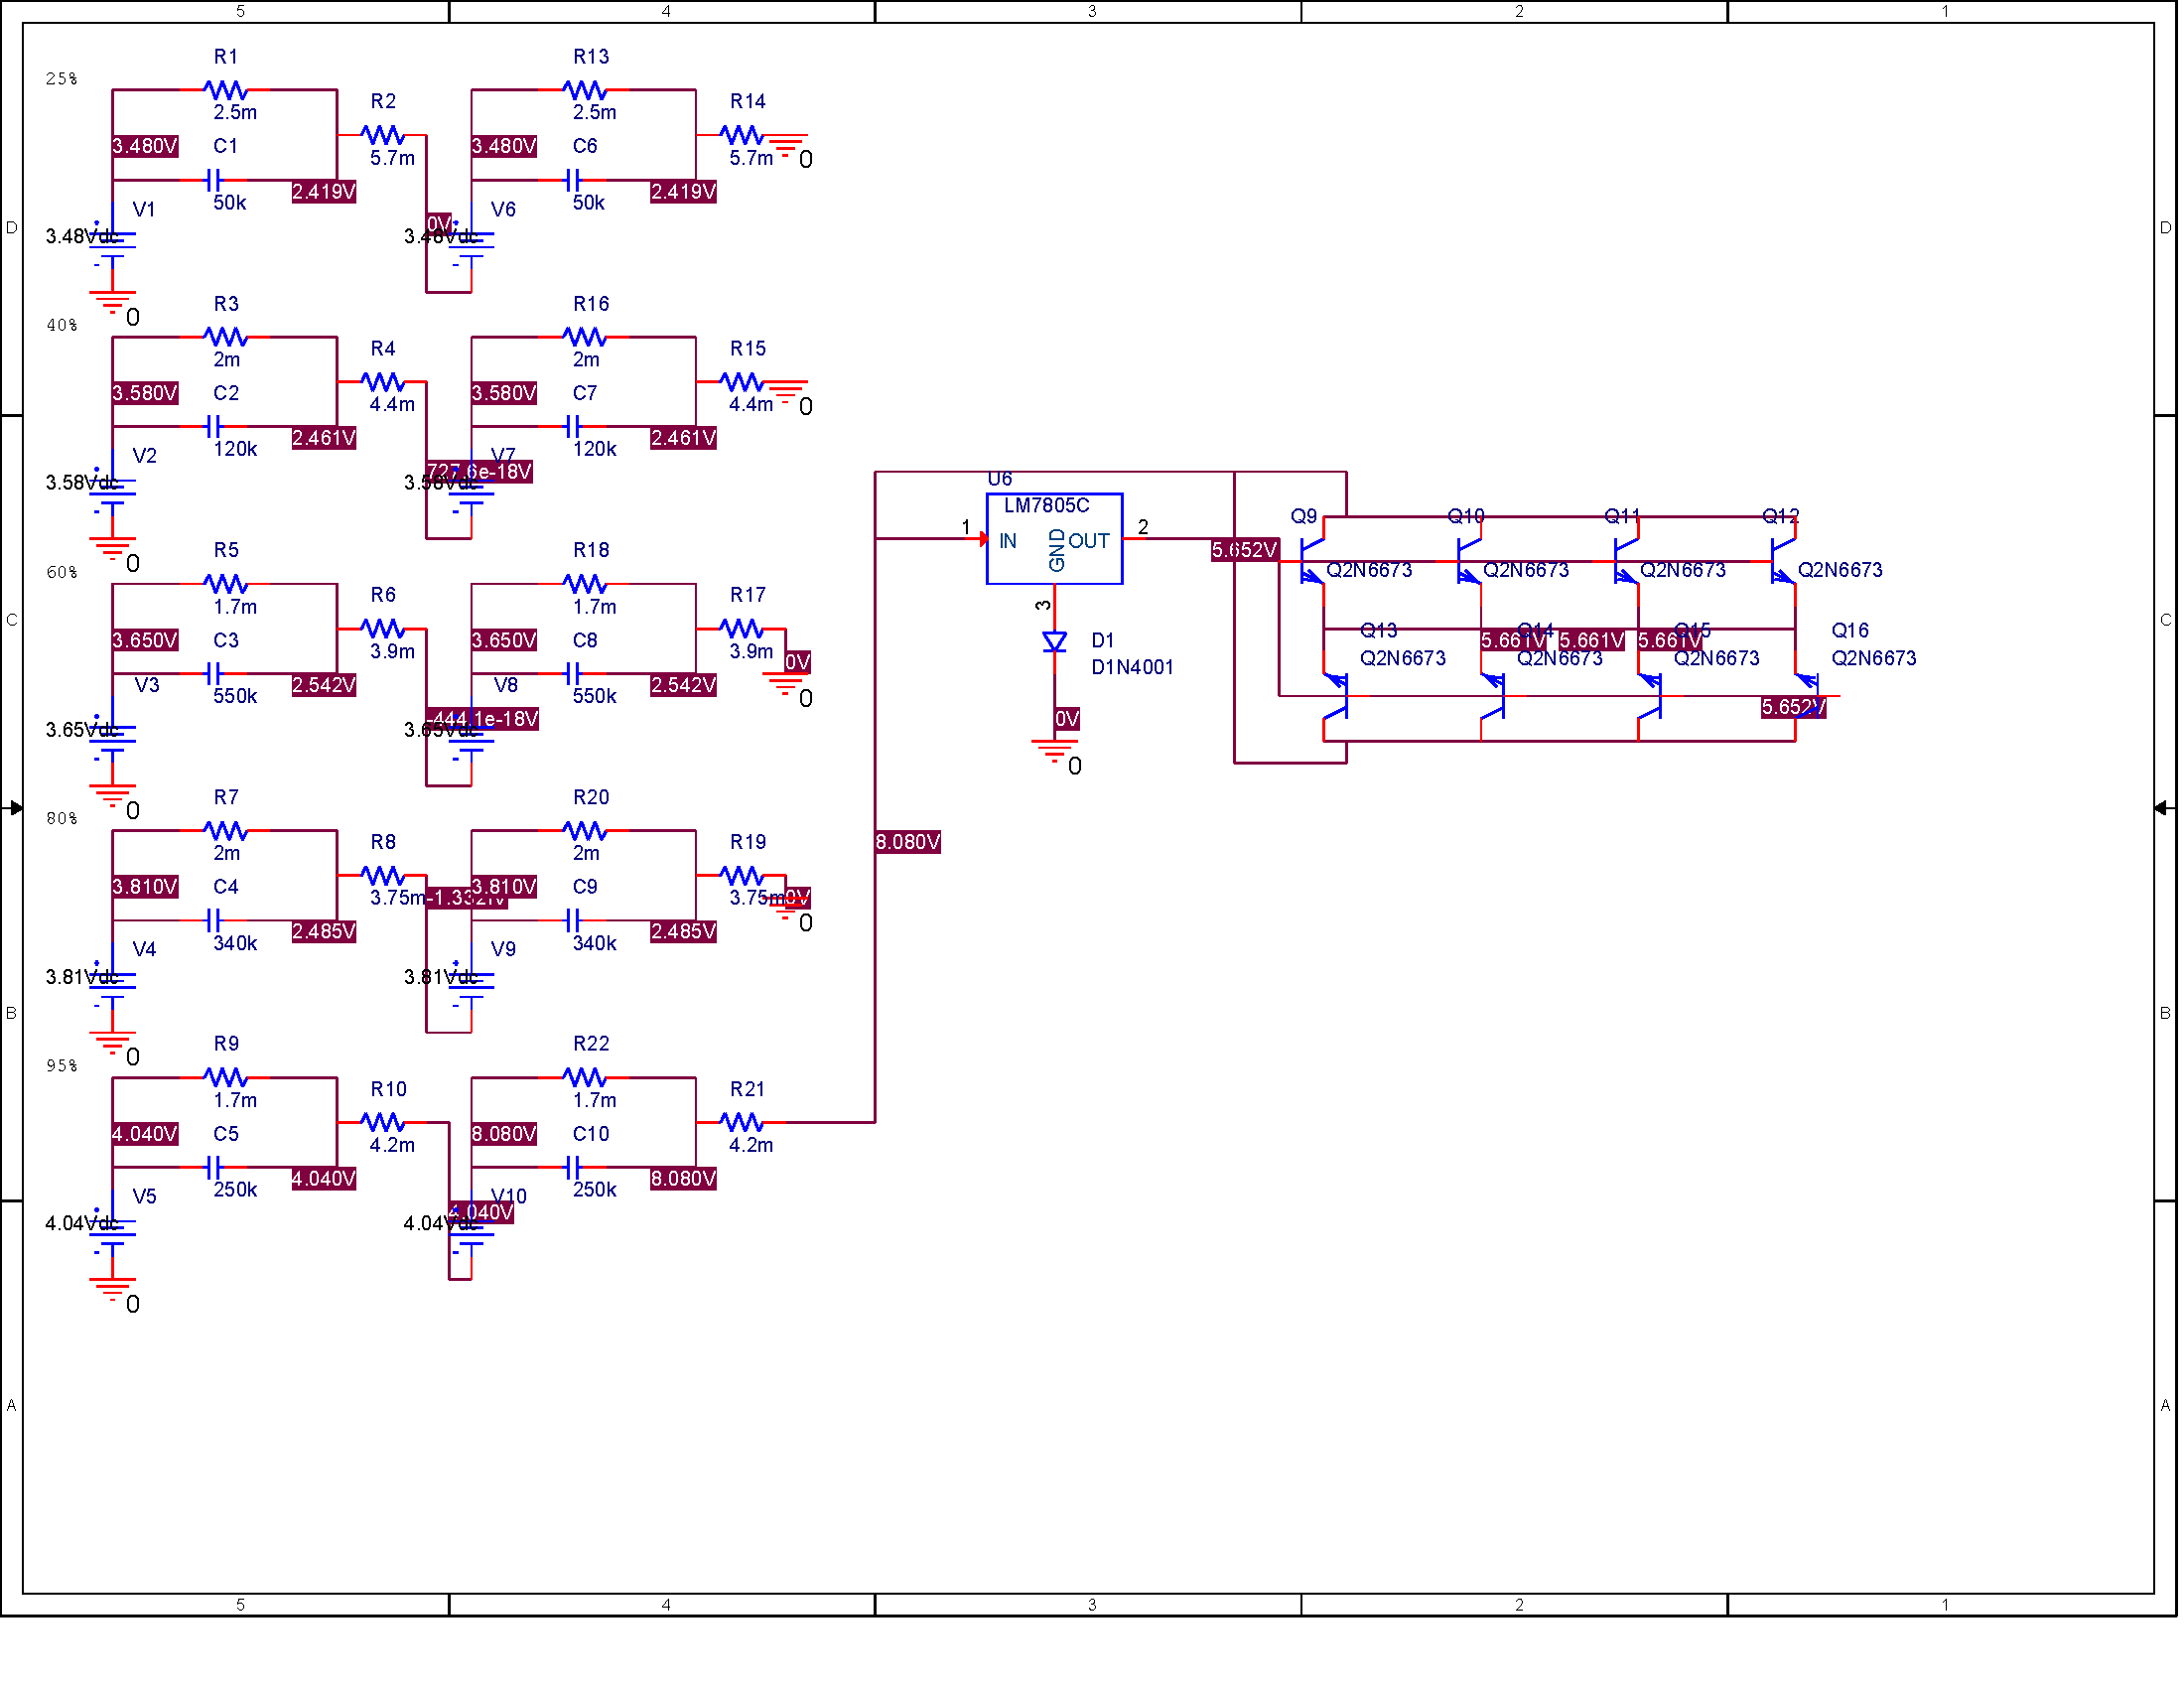
\includegraphics[width=\linewidth]{power.pdf}
  \caption{Low Voltage Power Circuit Schematic}
  \label{power-lv}
\end{figure}
There was no PSpice model available for the battery, so a model using experimentally determined voltages, resistances, and capicatances was implemented. The left hand side of the circuit is an array of different battery models for the same lithium cell at different charges, which are show on the top left. Pairs of identical models are connected in series because the circuit requires two lithium cells. The right hand side is the regulator circuit, composed of a simple LM7805 5V voltage regulator and several bypass power transistors to drive additional current. To ensure that the regulator circuit can provide steady voltage and that the batteries will stay within safe operating boundaries, the sets of batteries will be connected one at a time to the regulator circuit, and the regulator circuit will be connected to a load. Transient and steady-state characteristics of battery and regulator current and voltage will be measured to ensure safe and reliable operation.
\subsubsection{Linkage Analysis}
The are many metals that can be used to support structures. So it is important to look at the different strengths of each metal/alloy. When researching it was important to look at certain qualities. The following categories were important when searching for the correct metal to attach the tip and .
\begin{itemize}
\item Water Resistance
\item Yield Strength - the stress at which a specific amount of plastic deformation is produced, usually taken as 0.2 percent of the unstressed length.
\item Compressive Strength - the resistance of a material to breaking under compression.
\item Tensile Strength - the resistance of a material to breaking under tension.
\item Impact Strength - the capability of the material to withstand a suddenly applied load and is expressed in terms of energy.
\item Cost - how much for the total amount of metal we would need.
\item Machineability - how easy is it to work with the material
\end{itemize}
Below is a table with all of the data from the trade study on the materials.
\begin{figure}[!htbp]\centering
  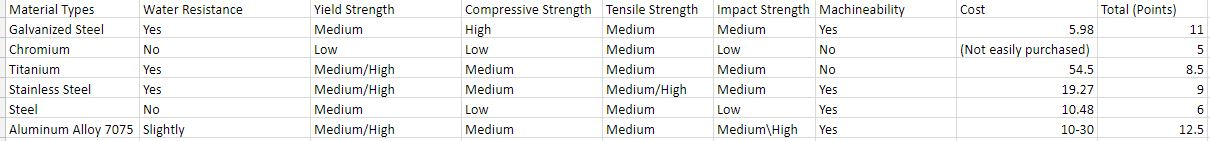
\includegraphics[width=\linewidth]{metals.JPG}
  \caption{Table with Metal Analysis}
  \label{metals}
\end{figure}
\newline
The results clearly show that Aluminum 7075 (T6) is the correct metal to support the board.

\subsubsection{Statics Analysis}
When producing a board, it is important to make sure that it has enough safety and security for consumers to ride without fear of board breaking. To make the board more modular, the tips were separated from the centerpiece, so that meant a supporting link(s) was needed to keep the board together. Using SolidWorks, the group 3D modeled the board and possible linkage types. The average pressure generated from a person is about 16 psi, so when running simulations, the assembly was tested at 18 psi to guarantee that it could support a vast majority of people. Through this testing it was apparent which linkages were more effective than others.
\newline
Below are some Linkage types that were tested. There were also, configurations using double the amount of links.

\begin{figure}[!htbp]\centering
\begin{minipage}{.5\textwidth}\centering
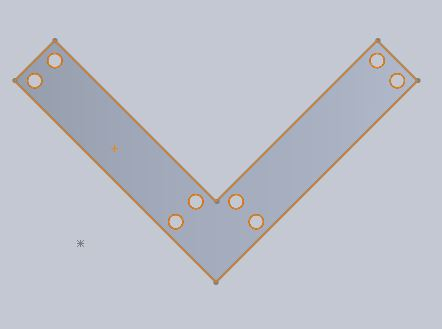
\includegraphics[width=.8\textwidth]{single-v.JPG}
\captionof{figure}{Single-V}
\label{singlev}
\end{minipage}
\end{figure}

\begin{figure}[!htbp]\centering
\begin{minipage}{.5\textwidth}\centering
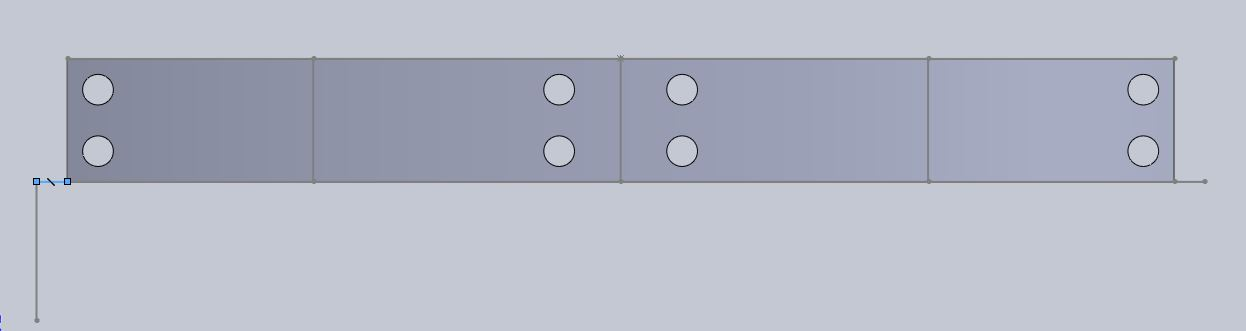
\includegraphics[width=.8\textwidth]{single-bar.JPG}
\captionof{figure}{Single-Bar}
\label{singlebar}
\end{minipage}
\end{figure}

\begin{figure}[!htbp]\centering
\begin{minipage}{.5\textwidth}\centering
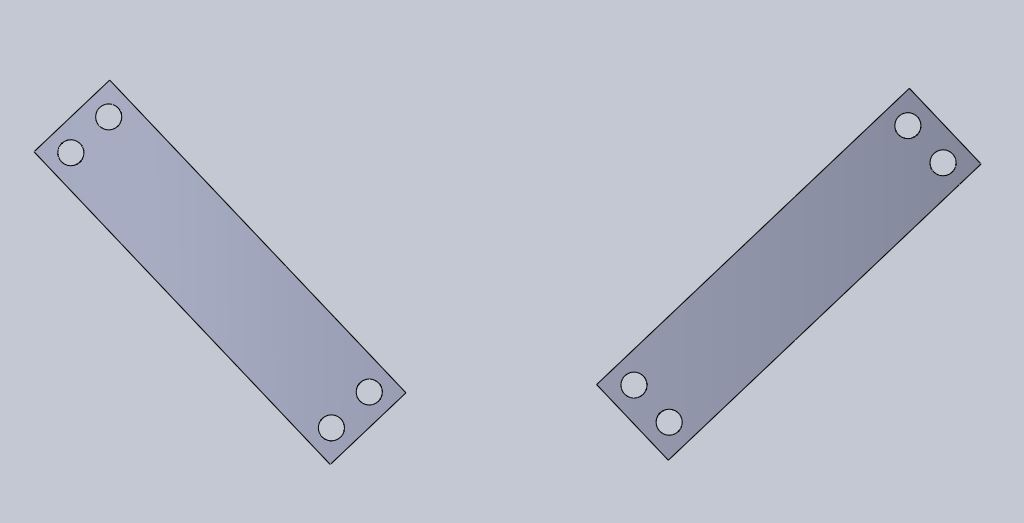
\includegraphics[width=.8\textwidth]{single-accent.JPG}
\captionof{figure}{single-accent}
\label{single-accent}
\end{minipage}
\end{figure}
\
The result of all the testing displayed that the Double V structure was the most structurally sound.
\end{document}
